\documentclass[10pt]{article}
\usepackage{subfigure,psfrag,epsfig,graphics,url,amsmath,amssymb,fancyhdr,cite,color}
\usepackage{multirow}
\usepackage{palatino}
\usepackage[font=small,format=plain,labelfont=bf,up,textfont=it,up]{caption}
\usepackage[small,compact]{titlesec}
\usepackage[margin=1in]{geometry}
\usepackage{setspace}

%\titleformat{\section}
%  {\normalfont\fontsize{10}{10}\bfseries}{\thesection}{0.5em}{}


%%%%%%%%%%%%%%%%%%%%%%%%%%%%%%%%%%%%%%%%%%%%%%%%%%%%%%%%%%%%%%%%%
% Hyperref stuff

%\usepackage[filecolor=black,citecolor=black,urlcolor=black,linkcolor=black,colorlinks,pdfpagelabels,pdfpagelayout=SinglePage,dvips]{hyperref}
%\usepackage{backref}
%\usepackage{breakurl}
%\renewcommand{\url}{\burl}

%% \renewcommand*{\backref}[1]{}
%% \renewcommand*{\backrefalt}[4]{
%%   \ifcase #1 %
%%     (Not cited.) %
%%   \or
%%     {\small\sffamily (Cited on page~#2.)}%
%%   \else
%%     {\small\sffamily (Cited on pages~#2.)}%
%%   \fi
%% }
%% \renewcommand*{\backrefsep}{, }
%% \renewcommand*{\backreftwosep}{ and~}
%% \renewcommand*{\backreflastsep}{ and~}

\newcommand{\TITLE}{CICI: UCSS: Usable Access Control for High Speed Research Networks}
\newcommand{\xxx}[1]{{\color{red} #1}}

%%%%%%%%%%%%%%%%%%%%%%%%%%%%%%%%%%%%%%%%%%%%%%%%%%%%%%%%%%%%

\newtheorem{definition}{Definition}
\newtheorem{task}{Task}[section]
\newtheorem{problem}{Problem}[section]

\usepackage[pdftex,hyperref,svgnames]{xcolor}
\colorlet{todo}{FireBrick} % FireBrick prints better than red
\newenvironment{todolist}[1][]
  {\color{todo}TODO: \em#1\begin{enumerate}}
  {\end{enumerate}}
\newcommand{\todo}[2][TODO]{\textcolor{todo}{[{\em #1: #2}]}}

\newcommand{\eg}{{\it e.g.}}
\newcommand{\ie}{{\it i.e.}}
\newcommand{\etal}{{\it et al.}}
\newcommand{\comment}[1]{}

\newcommand{\fp}{\vspace*{0.03in}\noindent}
\renewcommand{\b}{$\bullet$}
\renewcommand{\paragraph}[1]{\fp {\bf #1}}

\begin{document}
\date{}

% 6 lines per inch, per research.gov
\setstretch{1.05}

\pagestyle{empty}  % Danny: Suppresses all page numbers

\begin{sloppypar}
\thispagestyle{empty}
\begin{center}
{\large \bf \TITLE}
\end{center}

\fp {\bf Overvew:}

Many academic institutions have high speed research networks (HSRNs) that support up to 400 Gbps, enabling high bandwidth data transfers (e.g., sending large datasets within and across institutions) and low latency applications (e.g., AR/VR). Some of the data and code could be sensitive in nature. To prevent unwanted data exfiltration and theft of intellectual property, network administrators typically use off-the-shelf commercial or open-source security products. However, products like intrusion detection systems (IDS) may alert after some delay; on our 400 Gbps network, every second of delays in alerts, for instance, could result in 50 GB of data exfiltrated. Furthermore, products like firewalls and intrusion prevention systems (IPS) inspect traffic in-line — generally fast enough for traditional networks (e.g., 10 Gbps), but are too slow (or prohibitively expensive) for the 400 Gbps HSRN in our institution, restricting the bandwidth and introducing additional latency.

Our goal is to maintain the bandwidth and latency of HSRNs (>400 Gbps) while minimizing security risks, including unwanted data exfiltration and theft of intellectual property on the HSRNs. To this end, we propose to develop and deploy a new open-source system to address this issue using a researcher-in-the -loop approach to manage connections based on allow-lists on software-defined networks (SDNs), in a way that is usable and minimizes overhead to the HSRN. Using this approach, we will first evaluate and pilot this system within NYU's HSRN, and evaluate it with HSRN researchers and network administrators in terms of usability and performance, before working to deploy it with collaborators in the broader HSRN ecosystem.

The figure on the right illustrates our proposed technique. A researcher (e.g., who needs to transfer large files and/or who experiments with AR/VR) connects their computer [A] to the HSRN. All traffic to/from [A] goes through an SDN switch [B] (e.g., SONIC), which by default forwards the traffic to traditional in-line security products like firewalls and IPS devices [C]. This slow path is meant to handle traditional traffic such as OS updates and web browsing on [A]. Any system compromises on the HSRN will likely be detected on this slow path. When the researcher decides to utilize the high bandwidth and low latency of the HSRN, they visit a custom-built researcher-facing dashboard [D] to proactively indicate their intended destination (e.g., another computer running an experimental AR/VR application) or retroactively select an existing connection (e.g., an established data transfer to a Dept of Energy server) to be added to a temporary allow-list. The SDN controller [E] (e.g., based on the P4 Integrated Network Stack) implements this allow-list as flow-based rules on the switch [B], which then forwards the traffic via switch [F] to the fast path. To minimize human errors on the dashboard, switch [F] mirrors traffic on the fast path to Zeek [G], an IDS which analyzes the first N packets of each flow (handshakes), samples the remaining packets (encrypted), and alerts the controller [E] of suspicious connections. To complement Zeek, we save all Zeek logs to a Spark cluster on which to identify further anomalies, e.g., using RADAR and Spot.

\fp {\bf Intellectual merit:}

(1) A usable method (e.g., implemented at [D]) to help non-experts to proactively and retroactively add destinations or connections to the temporary allow list, augmented with traffic visualization and automated security advice. (2) A technique to balance the trade-off between security and accuracy of alerts (e.g., implemented at [G]) for different experimental needs. (3) Evaluation on actual HSRN at NYU in terms of security and performance, with a special focus on usability.

\fp {\bf Broader impacts:}

An open-source and extensible system for general HSRNs, allowing HSRN researchers to enjoy the full high-bandwidth and low-latency capabilities while minimizing security risks. A teaching tool for the intersection of usable security and software-defined networking.


\fp {\bf Keywords:} usability, security, networking

\pagebreak
\setcounter{page}{0}
\begin{center}
{\large \bf \TITLE}
\end{center}

\section{Introduction}

Many academic institutions have high speed research networks (HSRNs) that support up to 400 Gbps connections to data centers and the cyber infrastructure. To enable high bandwidth transfers research networks typically rely on data transfer nodes in the DMZ. However, in our case we have built a separate and dedicated network that reaches into research labs and research offices at up to 200 Gbps with redundant connections. This allows participating researchers to conduct high bandwidth data transfers, such as sending large datasets within and across institutions, and to support  low latency research applications, such as AR/VR and robotics. Researchers from many disciplines are benefiting from these high speed low latency transfers. . Active researchers on our own HSRN include AR/VR, Physics, Chemistry, Robotics, Electrical Engineering, Multimedia and Performing Arts, and Computer Science.

On HSRNs, much of the data and code is potentially highly sensitive in nature, and can include personally identifiable information about experimental subjects, key experimental data that could be of interest to national security, and intellectual property such as code, research data and results, and papers.

\paragraph{Threat Model}
An attacker could potentially access, exfiltrate, or disrupt (e.g., by modifying) sensitive research data and code on an HSRN or misuse the hardware connected to the network (e.g. DDNS). Such an  attack could originate from the Internet or from another host on the same research network (e.g., as a result of malware's lateral movement~\cite{ho2019detecting}).

\paragraph{Unique Challenges}
To prevent theft of intellectual property and unwanted data exfiltration, access, or disruption, network administrators typically rely on two solutions — both of which have limitations in HSRNs in general.

\underline{Challenge C1}: Network administrators often use off-the-shelf commercial or open-source security appliances. While this approach is common on general enterprise networks (typically ~10 Gbps), it likely incurs significant performance overhead on HSRNs (e.g., 400 Gbps). For instance, products like intrusion detection systems (IDS) may alert after some delay. On our 400 Gbps network, every second of delays in alerts, could result in up to 50 GB of data exfiltrated. Furthermore, products like firewalls and intrusion prevention systems (IPS) inspect traffic in-line — generally fast enough for traditional networks (e.g., 10 Gbps), but too slow (or prohibitively expensive for academic applications) for the 400 Gbps HSRN in our institution, restricting the bandwidth and introducing additional latency for researchers on the network.

\underline{Challenge C2}: Network administrators could manually create firewall bypasses for specific researchers. One technique, also known as Science DMZ~\cite{dart2013science}, would place scientific devices or data transfer servers on a separate high-speed network without any security checks. Although this approach places no restrictions on the bandwidth and latency, another compromised device (e.g., infected with malware while not on this network) could lead to data exfiltration on this isolated network. Alternatively, as in the HSRN at our current institution, network administrators create temporary firewall bypasses for specific use cases over predetermined periods. Researchers have to submit special requests to the network administrators regarding their proposed activities to bypass the security checks, including (but not limited to) the wall ports connected, the destination hostnames and ports, the amount of traffic, and the start/stop times. This is typically a manual process requiring efforts of both the researchers and network administrators — a likely bottleneck (sometimes in months) in a typically fast-paced and unpredictable research environment. Also, this manual process is prone to mistakes; we have seen cases where network administrators forgot to close ports in a timely manner, thus exposing the researchers to security risks.

\paragraph{Key Objectives}
We want to make HSRNs secure without compromising the networks' performance or the researchers' user experience. Our proposed research aims to satisfy the following three goals:

\begin{itemize}
    \item \underline{KO1}: Performance: Provide Researchers on the HSRN with access to  the unrestricted high bandwidth and low latency capacities offered by the network — thereby mitigating Challenge C1.
    \item \underline{KO2}: Usability: Require minimal efforts of researchers to access maximum network performance — thereby mitigating Challenge C2.
    \item \underline{KO3}: Security: Minimize the security risks to research data and the network presented in the Threat Model.
\end{itemize}




\paragraph{Proposed Technique}
We plan to develop, deploy, and evaluate a usable system that lets researchers temporarily and securely bypass security appliances (e.g., intrusion prevention systems, or IPS) for specific use cases — on their own with informed decisions. This system consists of three components:

A researcher-facing dashboard [D] for researchers to specify security bypass for their devices and use cases [A].
A software-defined network [E], [B], [F] that enables [F] or disables [C] security bypass for a particular application based on the researchers' action in [D].
A network measurement and analytics service to monitor, visualize and annotate and manage research traffic [G]. This service will also double as an IDS to catch potential mistakes by researchers in [D].

\begin{figure}[t]
    \centering
    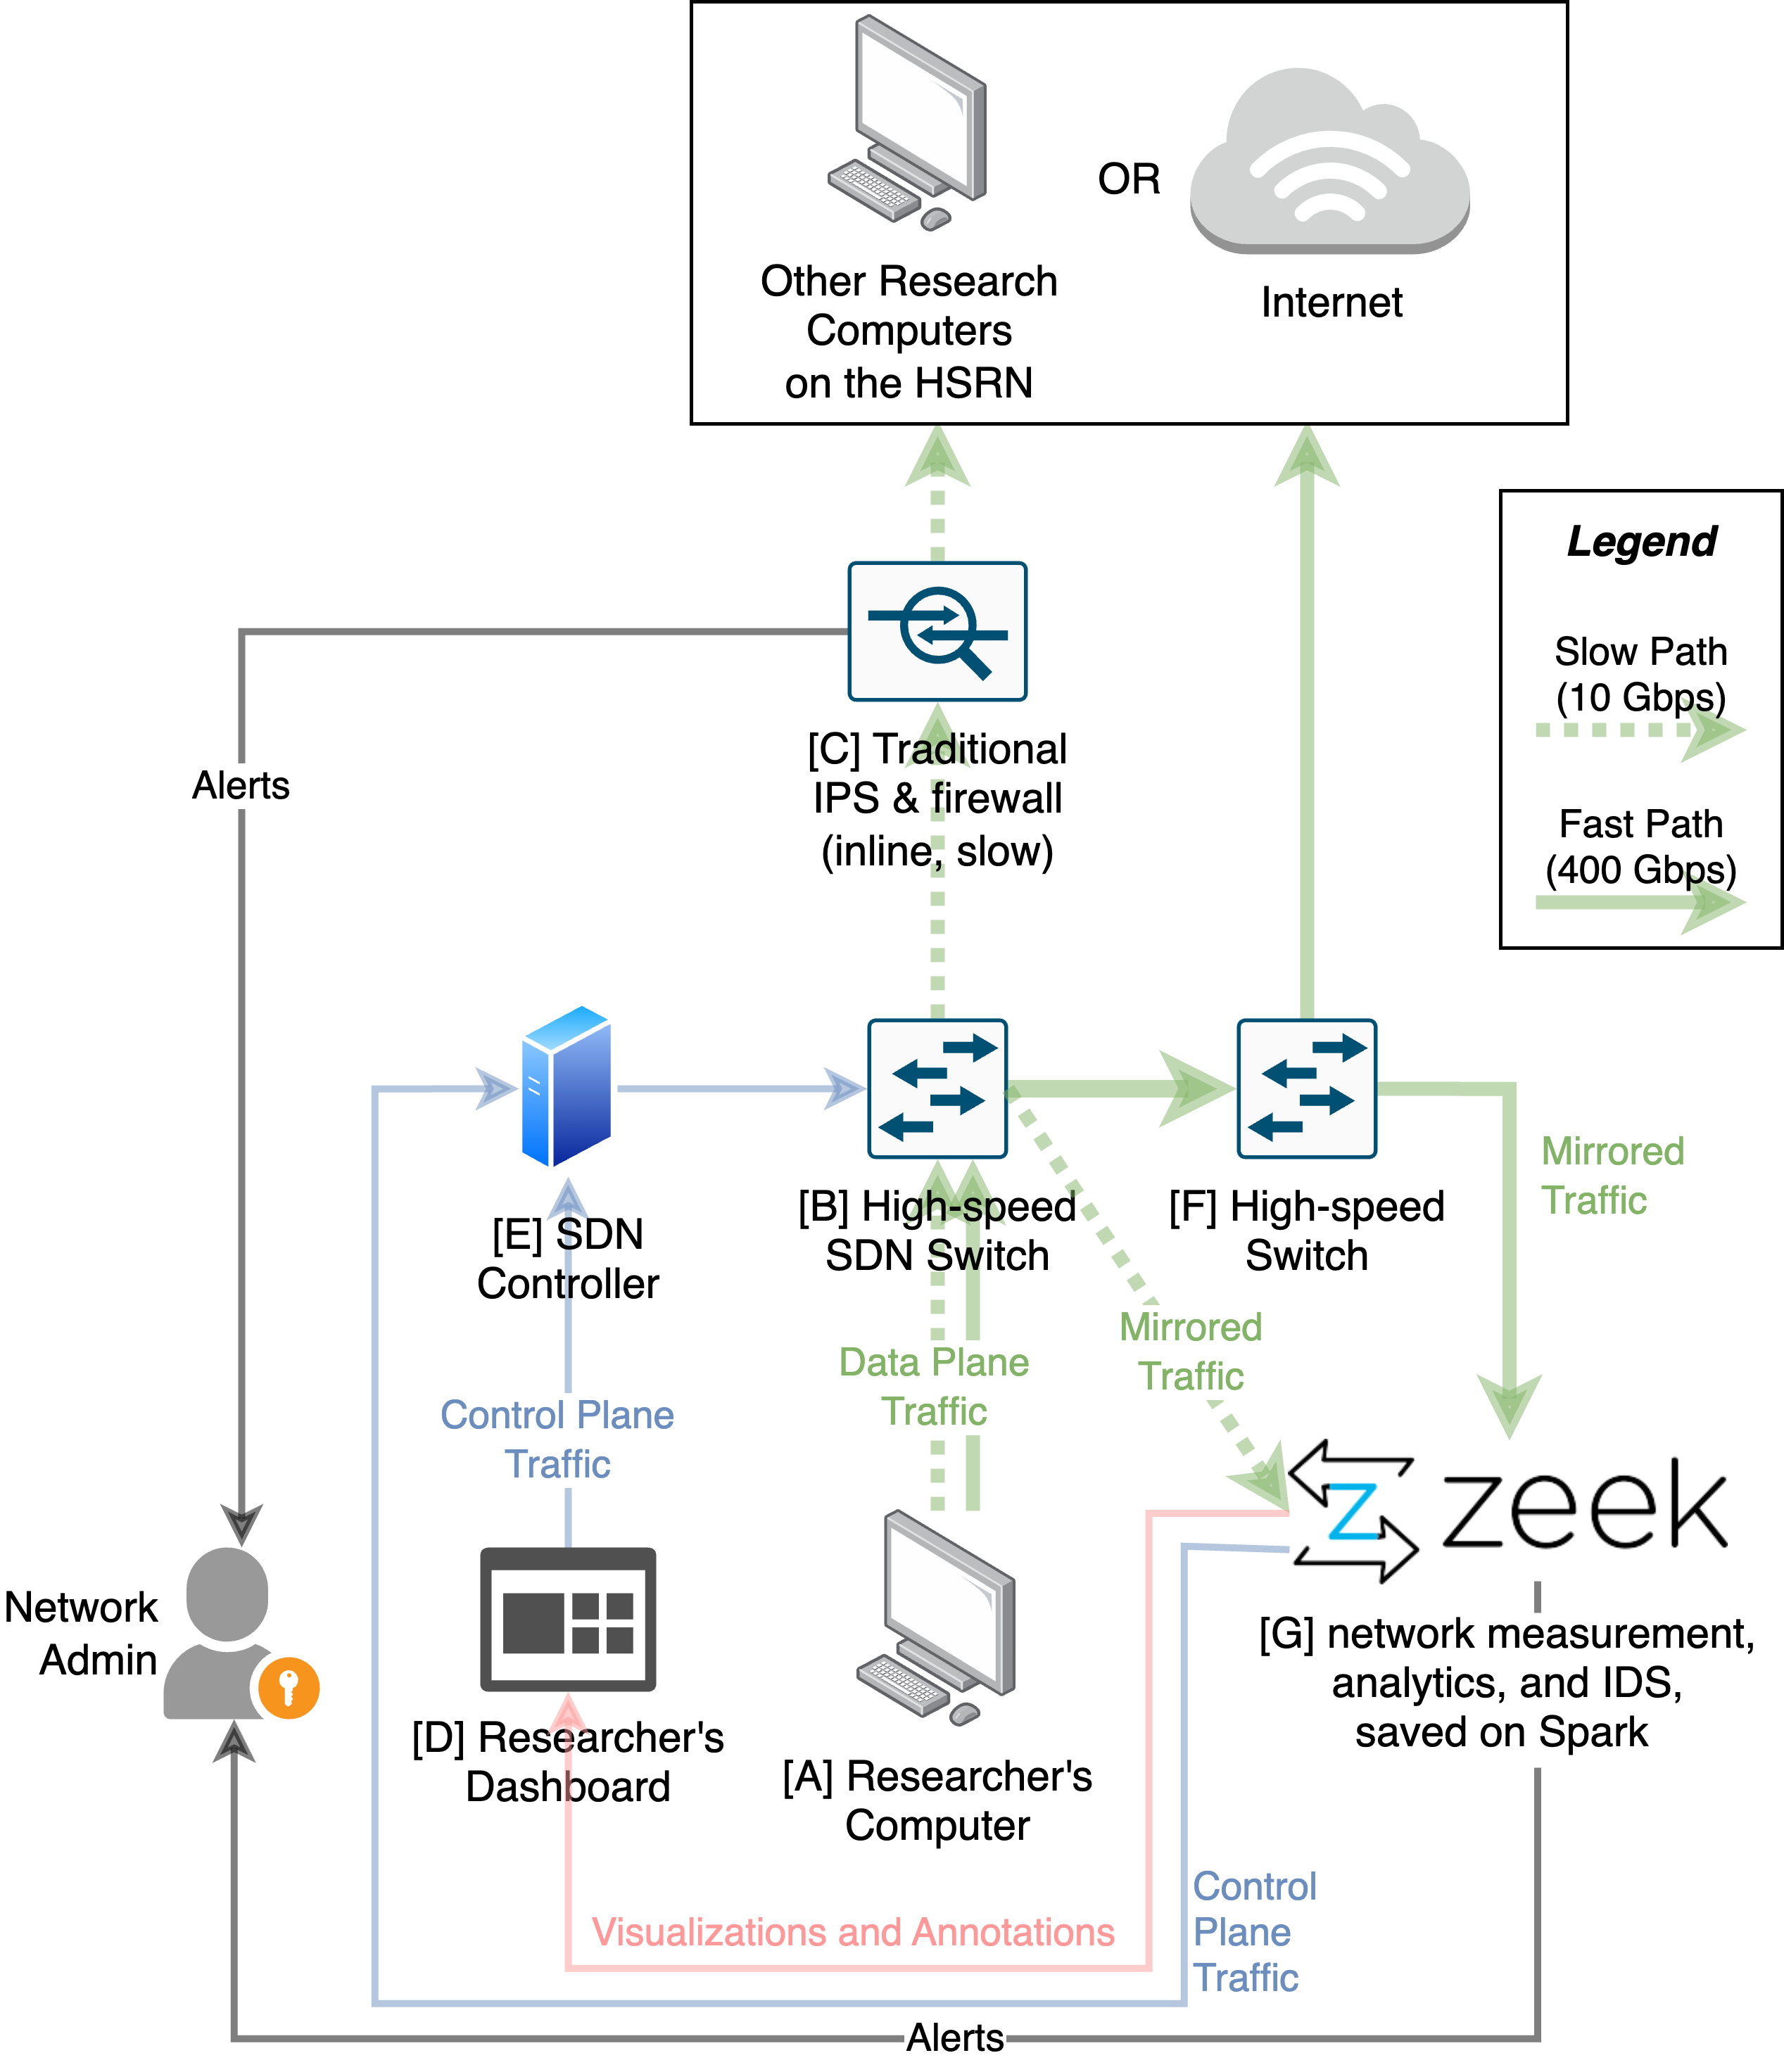
\includegraphics[width=0.6\linewidth]{figures/system.png}
    \caption{How our proposed system, i.e., [D] and [G], fits into a High Speed Research Network. To use our system, a researcher would first start their scientific workload (e.g., high-bandwidth data transfer or low-latency AR/VR application) on their device [A]. By default, all the researcher's traffic goes through traditional security middleboxes along the slow path, i.e., [A] to [B] to [C]. To enjoy the full benefit of the high bandwidth and low latency, the researcher visits a dashboard (proposed work) in [D] (an example of which is shown in Figure~\ref{fig:dashboard}), adds their scientific workflow to an allow list. The dashboard then adds a rule to the switch [B] via the control plane [E], which then reroutes the existing scientific workload through the fast path without any security middleboxes, i.e., [A] to [B] to [F]. We analyze the mirrored traffic at [G] to catch any potential mistakes from the researcher in configuring the allow list on the dashboard [D].}
    \label{fig:system}
\end{figure}

To illustrate how the proposed system works, we describe a sample interaction for a researcher in Figure~\ref{fig:system}. Here, a researcher connects their computer [A] to the HSRN to transfer 10 TB of data to a collaborator with the Dept of Energy (DoE). By default, all traffic, including the researchers' normal web traffic (e.g., web, checking emails, etc.) and the data transfer with DoE, go through the secure route of the network, where all packets are inspected by traditional security appliances such as IPS. This is a slow path (from [A] through [B] to [C]) (<10 Gbps), because  typical security appliances like IPS and firewalls [C] restrict the bandwidth and increase the latency.

After the researcher begins to transfer the files to DoE, they would open the dashboard [D] — a focus of our proposed work. Here, the researcher would see traffic data reports, visualizations and annotations, based on data-driven traffic analytics at [G] (example in Figure~\ref{fig:dashboard}). This traffic includes all network connections between [A] and the Internet, including the data transfer to DoE, along with other traffic on [A], such as web traffic. Based on the data, visualizations, and annotations, the researcher could select the DoE data transfer for security bypass for a given time or byte count (e.g., 10 TB). This action would cause the network controller [E] to automatically reroute  the existing DoE data transfer through the fast path (from [A] through [B] to [F]) (~400 Gbps) that bypasses security appliances (instead of the original slow path). The other non-DoE traffic is not affected and remains on the slow general network path.

\paragraph{Key Contributions}
Our novelty is in the usability of the proposed approach and the ability to integrate with existing state-of-the art HSRN and security appliances. This approach will allow researchers to utilize the high bandwidth and low latency of the high-speed network ( addressing Challenge C1), in a way that is instantaneous, streamlined (addressing Challenge C2), and secure. Our proposed work focuses on achieving this usability and integration. We defer anomaly detection (e.g., identifying data exfiltration or unauthorized access) to existing literature.

\paragraph{Team}
\underline{PI Dr. Danny Y. Huang} is an Assistant Professor at NYU's Department of Electrical and Computer Engineering. He is an expert on networking, security, and human-computer interactions. He has published papers on software-defined networking~\cite{huang2013high}, analyzing malware's network activities~\cite{huang2018tracking}, visualizing network traffic for non-experts~\cite{huang2020iot,thakkar2022would}, and understanding human behaviors in the context of security/privacy through user studies~\cite{major2021alexa,thakkar2022would,cruz2023augmented}.

\underline{Co-PI Dr. Robert Pahle} is a Senior Research Scientist at NYU Research Technology. He is on the development team of NYU's High-Speed Research Network. He is an expert on network deployment and operations, as well as open source development~\cite{corelink}.

\underline{Co-PI Dr. Justin Cappos} is an Associate Professor at NYU's Department of Computer Science and Engineering. He is an expert on production open source software deployments, e.g., Seattle Testbed, TUF, and in-toto~\cite{Cappos_CCS_2010, Samuel_CCS_2010, Torres_USENIXSec_2016, Nikitin_USENIXSec_2017, in-toto-paper,Zhuang_NSDI_2014,Kuppusamy_NSDI_2016}.

\paragraph{Summary}
Our proposed work will benefit HSRNs at NYU and beyond, which are popular among scientists who need a high-bandwidth, low-latency computing environment. We will make HSRNs more secure and usable without compromising the networks' performance. This simplicity promotes collaboration and innovations across disciplines, as researchers will be able to keep and share their sensitive information safely without significant administrative overhead to achieve security




\section{Broader Impacts}\label{sec:impacts}


Our initial design and deployment is based on NYU researchers. But we can definitely go beyond.

// From: Jeremy
-Facilitating
-improved monitoring, management and security of academic networks and research
data.
-increased researcher awareness and responsiveness to network and data security.
-research requiring large data transfers and low latency applications.
-research collaboration across institutions and with private and public partners.
-intra- and inter- institution collaborations around open source community user access
management for high speed research networks.

-Leveraging
-current NSF investments in research.
-regional/national infrastructure initiatives such as NAUTILUS, FABRIC, etc.
-NSF funded cyberinfrastructure at many institutions.

Benefiting actual HSRN users. NYU researchers are very happy. We have letters from them. Multiple departments. Co-PI Pahle, already a part of NYU Research IT, will make sure to keep it running.

Benefiting beyond NYU. Proposed license: publicly available; MIT, can be modified for other environments. Beyond NYU, generalizable across different HSRN. If no SDN, [E] can be a system to write rules on switches. Our approach is agnostic of security appliances. Open-source Zeek. Useful for other institutions.

Workforce development. Lowers the barrier for network administrators. Allows existing employees (some of whom are students) to troubleshoot and learn. Easier to train folks to maintain.

Education. Classroom use. Good teaching tool to visualize traffic on an enterprise research network. Both PI Huang and Co-PI are a part of the Center for Cyber Security. Both teach network and security classes.

Community engagement. Open source. We welcome community contribution. Co-PI Cappos is an expert on mobilizing the open-source community.




The project has two broader impact goals: (1) improving DNS privacy through
the deployment of new protocols in practice; (2) educating a diverse set of
next-generation computer scientists. In this section, we highlight
initiatives toward each of these goals.

\paragraph{Improving DNS privacy in practice.}
We aim to transition research results to practice, through
continued engagement in standards bodies (\eg, Internet Engineering Task
Force) and operators groups (\eg, North American Network Operators Group) and
through
integration with browsers (\eg, Firefox, Tor
Browser) and open-source stub resolvers (\eg, Stubby). We have created an
initial prototype implementation of a distributed DNS stub resolver as an
extension to Facebook's open-source DoH proxy~\cite{fb-doh-proxy}. In this
project, we will aim for more comprehensive and widespread open-source
deployments, building on early discussions with both Mozilla and the Tor
Project. The PI plans to continue to engage with the IETF DNS Privacy
(DPRIVE) working group~\cite{dprive} to continue to develop and propose standards based on
research outcomes.

\paragraph{Student and researcher mentorship.} To improve education in ways
that broaden participation in computing, the PI will create interconnected
programs that merge sustained engagement with diverse students in Chicago
Public Schools, provide summer research experiences, and carefully scaffold
these research experiences with on-ramp immersions that lower barriers to
participation.

To provide meaningful research experiences to students, PI Feamster will
annually mentor a diverse group of students, ranging in level from high school
to post-graduate as a way to encourage future participation in computing
programs. These efforts will benefit from engaged partnerships with
organizations to aid in recruitment and tracking student outcomes: (1)~The
UChicago Collegiate Scholars Program; (2) the Office of Special Programs (OSP)
College Prep; (3)~The Fisk-Vanderbilt Master's-to-PhD Bridge Program for
underrepresented students.

The PI has a successful track record in mentoring women and underrepresented
minorities. For example, he currently advises two female Ph.D. students, one
of whom is also an underrepresented minority. These students have won research
awards; Annie Edmundson won the 2016 ACM Student Research Competition at ACM
SIGCOMM. The PI is involved with various efforts around the department to
increase inclusion and diversity.  Feamster also regularly involves
undergraduate students in research, both during the academic year and summers.
PI Feamster mentored three undergraduate students (including one female
student) in Spring 2017 on a home network IoT inspector project, which
resulted in a submission to the Federal Trade Commission's IoT Home Network
Challenge~\cite{iot-monitor-ftc}, a presentation to the Coalition for National
Science Funding~(CNSF)~\cite{cnsf2017-iot}, and presentations to Congress,
including Senator Markey~(MA) and Representative McNerney~(CA-09).  In
Summer~2017, Feamster hosted several undergraduates for research, including
Jessica May, a female undergraduate student from the University of Nebraska.
The research performed by undergraduates has often resulted in peer-reviewed
publications (including as first author on top-tier venues such as SIGCOMM and
IMC).  Many of the PI's undergraduates have continued either to top graduate
programs or highly desirable companies. Of those, in the past few years, PI
Feamster has worked with six female research assistants.  Another aspect of
education is providing students with internship opportunities The PI will seek
out real-world opportunities at government offices, companies, and civil
society organizations to train students.  When hiring, the PI will follow best
practices for encouraging diversity in hiring, including interviewing a
diverse set of candidates and advertising in forums that serve
under-represented minorities (\eg, Tapia and Grace Hopper).

\paragraph{Outreach to under-represented high school students.}
To further engage under-represented minorities in the project, the PIs will
integrate results from this project into K-12 education programs, such as the
University of Chicago's Upward Bound program, where PI Feamster currently
teaches an ``Applications of Machine Learning to Networking'' summer course to
under-represented students across the Chicago Public School system.
This program  has allowed the PI to directly engage with high
school students  enrolled in Chicago Public Schools (77\% economically
disadvantaged and 83\% underrepresented minority) and their parents for an
annual series of 10 seminars and 6 weekend workshops hosted at UChicago on our
project's key themes.
This on-ramp will introduce core computing
skills, build an understanding of the research process (e.g., how to ask a
good research question), and help the students set productive routines in
unstructured environments.  Perhaps more importantly, it will help build a
community and support network among each year's student cohort and the larger
team of co-PIs through near-peer mentoring and informal interactions.
Following this immersion, the students will work for the rest of the summer
with their respective co-PIs.

\paragraph{Course development.} PI Feamster is currently teaching a research
seminar on the Internet and free expression and drafting a book on the topic.
The PI will develop new course materials pertaining to DNS privacy, both for
courses at the University of Chicago and in the form of publicly accessible
course material, as in Massive Open Online Courses (MOOCs), which PI Feamster
has developed in the past. The PI already teaches several courses where topics
from the research may be integrated, including undergraduate Information
Security, Networking, Many University of Chicago undergraduate students
also perform independent research. The PI will generate project ideas for
independent work projects and undergraduate theses and will invite students to
undertake these projects.


\paragraph{Integration into educational programs.}
Ultimately, we aim to integrate the data that we gather into educational
materials and courses. Examples include Machine Learning for Public Policy;
Data Science, Social Science and Public Policy; and the Machine Learning
Concepts and Applications course that PI Feamster teaches in the University of
Chicago's Upward Bound, a college readiness program for under-represented
minorities in the Chicago Public School system. The Center for Data and
Computing will also involve industry partners in specific projects and
engagements with students through the Chicago Data Science and Technology
Clinic, a new program that matches computer science and computer science
masters students to longer-term projects, such as those we describe in this
proposal.
The PI will also convene student
activities, including hackathons, that leverage the outputs from the proposed
research and are geared towards outputs with broader impact.  We plan to help
organize local student activities that help students prepare
entries for these competitions at the Center for Data and Computing (CDAC), as we have in the past.



\begin{figure}[t]
    \centering
    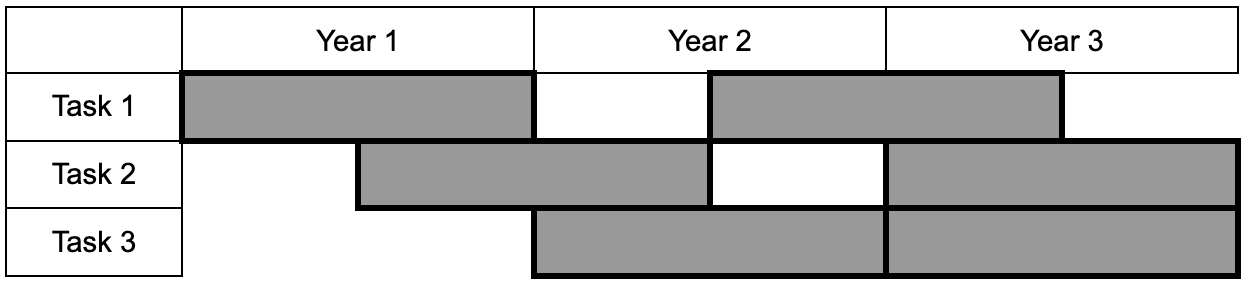
\includegraphics[width=0.6\linewidth]{figures/timeline.png}
    \caption{Timeline.}
    \label{fig:timeline}
\end{figure}


\section{Management Plan and Timeline}\label{sec:management}

PI Huang will manage all aspects of this project. The project will involve
graduate students and research staff who will help with the implementation of
the project, as well as sustaining the software over time and transferring the
data and systems to other organizations, as described in
Section~\ref{sec:impacts}. We envision that the tasks of this project will
proceed roughly in phases, in order, with some overlap as appropriate. As illustrated in Figure~\ref{fig:timeline}, we will proceed with Tasks 1, 2, and 3 in order, with some overlap in the middle to allow for continuous improvement and feedback. Once we deploy, we will return to Task 1 and Task 2 again to further improve the system based on preliminary deployment in Task 3. We hope to achieve full-scale deployment by the end of the third year, while continuously running user studies (Task 1) and fine-tuning our traffic annotations and anomaly detection (Task 2).

\section{Results from Prior NSF Support}

\subsection*{Danny Yuxing Huang}
PI Huang is supported by NSF Award 2219867 ``Privacy-preserving IoT Analytics and Behavior Prediction on Network Edge.'' This has given him the experience of analyzing massive amount of network traffic and conducting machine learning, such as anomaly detection, on network flows.


\subsection*{Robert Pahle}
Co-PI Pahle is supported by NSF Award 2232817 ``DataStorage: Distributed, Fast, Scalable Infrastructure for Emerging Media Research Data.'' This has given him extensive experience in conducting experiments on NYU's high-speed research network infrastructure and collecting preliminary data on workloads and user experience.



\subsection*{Justin Cappos}
Co-PI Cappos has a history of deploying software widely in practice and then
tackling the research problems that arise. PI Cappos has designed improved
security models for Linux package managers~\cite{Cappos_CCS_2008}, cloud
container systems~\cite{Kuppusamy_NSDI_2016, Kuppusamy_USENIX_2017}, and
version control systems~\cite{Torres_USENIXSec_2016} and in all cases
deployed these new models into use across millions of devices.

Due in large part to NSF support (1513457, 1444827, 1223588), PI Cappos's
research advances have been published in top venues in
security~\cite{Cappos_CCS_2010, Samuel_CCS_2010, Torres_USENIXSec_2016, Nikitin_USENIXSec_2017, in-toto-paper},
networking~\cite{Zhuang_NSDI_2014, Kuppusamy_NSDI_2016},
education~\cite{Cappos_SIGCSE_2009, Cappos_SIGCSE_2014, Hooshangi_SIGCSE_2015},
software engineering~\cite{Rasley_ISSRE_2015, Oliveira_ACSAC_2014,
Gopstein_FSE_2017},
and systems~\cite{Li_USENIX_2015, Li_USENIX_2017, Kuppusamy_USENIX_2017}.

\textbf{Broader Impacts:} PI Cappos emphasizes the transition of work into practical use and had
substantial success on that front.  For example, NSF
grant 1345049 ``NSF TTP: Securing Python Package Management with TUF''
provided a year of funding to transition TUF into use, leading to its
standardization by Python and use by
DigitalOcean, CloudFlare, DataDog, RedHat, VMware, Microsoft, Google,
IBM, Amazon, and Docker.
Overall, PI Cappos has
transitioned research into production use in a wide array of widely used
software including Git, Python, popular cloud environments, automobiles,
and most Linux distributions.

PI Cappos also has substantial experience with using his research in the
classroom.  His Seattle testbed (supported by NSF grants 1405904,
1405907, 1547290, and 1205415) has been used in about 100
security and networking classes.
He built a core community from the early adopters, through which
he developed a group of colleges that use the existing educational
materials~\cite{NWDCSD}.

The PIs have also used NSF support to increase impact with faculty at high
schools and non-research institutions.
To support the educational component for NSF grant 1054754,
PI Curtmola has organized a 4-day professional development workshop
for high school teachers~\cite{asee14,ccwt14}, helping them
develop curriculum units to be integrated into high-school subjects.

PI Cappos has been teaching a computer
security summer camp for college and high school faculty through NSF
awards (NSF 1241653: ``NSF DUE: Building Cyber Security Capacity in Two Year
and Four Year Colleges'' and NSF 1407161: ``NSF RET in Engineering and
Computer Science Site: Research Experience and Training in Cyber Security for
Pre-College Teachers'').  This has provided invaluable connections with
educators who use the PI's educational modules.  Such contacts provide a
natural mechanism that he has used to successfully disseminate educational
modules~\cite{Cappos_SIGCSE_2014, Hooshangi_SIGCSE_2015}.












\pagebreak
\setcounter{page}{1}
\bibliographystyle{abbrv}
\bibliography{ref,rfc}

\pagebreak
\setcounter{page}{1}
\begin{center}
{\large \bf \TITLE}
\end{center}

\begin{center}
    {\bf Data Management Plan}
\end{center}






\noindent {\bf Data Types:} Several types of data will be generated by this project:

\begin{enumerate}
\item Information about data artifacts,
\item Specifications and code for sys,
\item Technical reports and scientific articles
\end{enumerate}

The first item is all public information we are retrieving and collating, so
we will keep the data we gather public.  The second item will be generated
by our team (as we write the software) and will be done in a public GitHub
repository.  The third item(s) will be generated initially privately for
submission to potentially anonymous venues but then published afterwards.  We
do not anticipate any data we use in this research will be private and we
will make it all available for use by researchers.


%While constructing \sysname, we will gather enough information
%handle any abuse complaints or similar issues.   To this end, we gather and
%collect flow information in a similar manner to PlanetLab's PlanetFlow
%service.
%We also log various types of experimenter use for our testbed for
%debugging and software improvement purposes.
%We also will log information to allow us to understand the size and diversity
%of our user base.   We log sufficient information to improve and understand
%how developers are using our clearinghouse and our nodes.
%
%As discussed in the proposal, the Android app for \sysname itself
%has privacy and data management protections built throughout the technical
%design.  Uses of sensor data
%must pass through the experimenter's IRB procedure as was already approved by
%an extensive IRB review at our institution.
%However, non-sensitive access (such as for experiments
%that do not specifically want sensor data)
%will proceed without undue restrictions.   The security layer functionality
%enables us to write customized access control and data flow restrictions for
%researcher experiments as is needed.


%The experimenters that use our testbed will be responsible for generating and
%managing their own data.   This will be done according to the policy set out
%by their data management plan / IRB.


\noindent {\bf Legal and Ethical Issues:} Due to adherence to IRB policies, no specific
ethical or legal issues are anticipated to arise in this work.
The PIs (from NYU, Purdue, and NJIT) will request IRB approval in the case
where user focused data collection is desirable. In addition, the data
generated through this research is not expected to be covered by any
copyright or database right.

%Our testbed restricts the set of
%things a researcher can do to prevent things like source address spoofing
%and ICMP packets (both are major sources of complaints on PlanetLab).
%As we will utilize some of the functionality from the Seattle testbed, we
%will also port their emergency stop mechanism over.  In the case where there
%is a complaint of abuse, we can use this mechanism and then contact the
%experimenters to understand more about whether the experimenter use was
%appropriate or not.

\vspace{5pt}
\noindent {\bf Access, Data Sharing, Reuse:} All of the code from this project is and
will continue to be released under a permissive open source license such
as Apache 2.0 or MIT.
The project's website is hosted on GitHub and provides access to the prototype
implementation, documentation and system specification.
The source code is hosted on a public GitHub repository.
Project results will be widely
disseminated to the community through project website, conference publications,
journal articles, NSF annual meetings, annual reports, and similar methods.

Dissemination to general public will be achieved through media
outlets, magazine publication, and presentation in public forums.
Broad discussion of this platform is key to growing and diversifying our
user base.   The PI has cultivated relationships with print and television
journalists that has broadened the visibility of other projects.   These
relationships will be utilized here to evangelize and grow the user base of
XXX.

The data and metadata collected about software is provided voluntarily by the
entities providing that software and will be used to determine the
trustworthiness of the software that is made available to the end user.

%We will build a web-based version for the tool that will be used by project owners to design and
%generate supply chain layouts. The tool will capture usage information
%when creating supply chain layouts.
%We will also request feedback from users about the usability and features
%available in the tool. All of this information will be used internally by the project team
%to improve the usability of the layout creation tool and will not be shared with any other parties.
%Users of the tool will be informed about what kind of of information
%is collected, for what purpose it is being used, and will be asked for consent before using the tool.

\vspace{5pt}
\noindent {\bf Data Standards and Capture Methods:}
As stated in the proposal, Observers will capture information.  In the
case that it is desirable, user feedback will be collected
using a standard web-based user
interface.
%Data will be collected from
%user studies via a standard web-based user interface.
%node manager and security
%layer / reference monitor interposition in experiments.

We will continue to use standard development tools like GitHub to manage
code, document the project, and synchronize effort across developers.


\vspace{5pt}
\noindent {\bf Short-term and Long-term Data Storage and Data Management:}
To date, the amount of data stored by this work can fit on a standard
server.  Although the anticipated data volume is hard to evaluate, we
estimate that a 2TB drive will suffice.

No specific security measures will be needed
concerning data storage. In general, storage will follow the procedure used in
Professor Cappos's Secure Systems Lab at NYU.

\begin{enumerate}
\item System and measurement data will be stored and kept online for three
years beyond the project life.
\item Source code will be stored on both the workstations and servers. Git
is an adequate tool to achieve this long-term archiving task.
\item Electronic copies of reports and articles will be kept on multiple
devices, such as cloud document storage, laptops, desktops, and servers.
\end{enumerate}

\vspace{5pt}
\noindent \textbf{Authorization for data access and protection of data:}
In the case where we do elect to conduct a user study,
user data will be stored in a format in which personal
identifiable information such as names will be replaced
by a user ID to protect user privacy.
Volunteer participation and user study data will be kept
in a secure location as per the IRB
instructions.
After the data
collection phase, the data will be moved into storage on
machines that have limited connectivity to the Internet, in order to
minimize the risk of data theft.


\vspace{5pt}
\noindent {\bf Resources:}
The PIs will supervise and be responsible for implementing and maintaining this
data management plan.  Senior personnel, students, and open source contributors
will be given a briefing on this plan prior to obtaining write access to the project's
GitHub repository. This will ensure a smooth implementation of the plan.






















\pagebreak
\setcounter{page}{1}
\begin{center}
    {\large \bf \TITLE} \\
    {\bf Facilities, Equipment and Other Resources}
\end{center}



\section*{Resources from NYU Research Technology}

The PI and both co-PIs have access to the following resources from NYU Research Technology. In particular, co-PI Pahle is a part of NYU Research Technology and helps the development and maintenance of the High Speed Research Network.


\paragraph{NYU Global Network}
New York University (NYU) comprises three degree granting campuses (New York City (NYC), Abu Dhabi (AD), and Shanghai), 18 schools and colleges, and 11 study away sites throughout the world. In NYC alone, NYU supports dozens of buildings on its Washington Square Campus; a “health corridor” that includes NYU Grossman School of Medicine, College of Dentistry, and College of Nursing on the east side of Manhattan; the Institute of Fine Arts on Manhattan’s Museum Mile; and in Brooklyn, the Tandon School of Engineering on NYU’s campus at Metrotech and a new facility at 370 Jay Street, which houses a broad array of media, technology, arts, and applied urban science programs.

Throughout these facilities, NYU faculty, students, and staff have access to advanced research and instructional computing resources administered by the Research Technology division of NYU IT. These resources include High Performance Computing (HPC) and Big Data clusters, a dedicated High Speed Research Network, parallel and archival file systems, a wealth of open source and commercial software, as well as support, training, and consultations on how to best use the available resources.



\paragraph{High Speed Research Network}
In addition to the NYU global campus network, NYU-Net, NYU has made a significant infrastructure investment to create a High-Speed Research Network (HSRN) to link its researchers with central supercomputing and data center resources, and with external collaborators via the New York State Education and Research Network (NYSERNet) and Internet2. The HSRN is dedicated to research community needs and is separate from the 40 gigabit/second academic NYU Campus Ethernet Network (NYU-Net). HSRN Phase I in summer 2020 connected three key research facilities with the High-Performance Computing Clusters and other institutional research facilities in the NYU Research Computing Data Center (RCDC). Individual computers can be configured to connect to the HSRN via copper at up to 10 gigabit/second (20 with redundant active/active configuration), and via optical fiber at 100 gigabit/second (200 gigabit/second redundant in an active/active configuration). HSRN Building level connections are made via a dual 400 gigabit/second to the network core. The phased HSRN implementation will scale to connect additional buildings and research labs throughout the university, and will provide additional access to High Performance Computing resources, centralized storage for backup, disaster recovery, and University level Digital Archiving/Data Management and Repository services. A research faculty governance group provides oversight and input regarding operations, with NYU IT providing HSRN security, monitoring, consultation and managing the connected computational and data center resources.


\paragraph{High Performance Computing}
The NYU New York City High Performance Computing resources include:

The central NYU HPC cluster, nicknamed Greene, consists of 4 login nodes, 524 “standard'' compute nodes with 192GB RAM and dual CPU sockets, 40 “medium memory” nodes with 384GB RAM and dual CPU sockets, and 4 “large memory” nodes each with 3TB RAM and quad CPU sockets. All cluster nodes are equipped with 24-core Intel Cascade Lake Platinum 8268 chips. The “standard” and “medium memory” compute nodes (a total of 564 nodes with 27,072 processing cores) are Direct Water Cooled (DWC) nodes by operating two Cooling Distribution Units (CDUs). DWC allows us to run the CPU at Turbo frequency of 3.7GHz nodes while we maintain operation of all processing cores. The Greene cluster also includes 65 compute nodes each equipped with 4 NVIDIA RTX8000 GPUs (a total of 260 RTX8000 GPUs), 10 nodes equipped with 4 V100 GPUs (a total of 40 V100 GPUs), and 9 nodes equipped 4 A100 GPUs (a total of 36 NVIDIA A100 GPUs). All cluster components are interconnected with an Infiniband (IB) fabric in a non-blocking Fat-tree topology, consisting of 20 core switches and 29 leaf switches. All switches are 200Gbps HDR IB switches while each compute node connects to the fabric using an HDR-100 adapter. The cluster comes with 7.3PetaBytes of usable data storage running the GPFS file system. Greene was ranked \#271 in the top500 list that was published in June of 2020.

The NYU HPC team in NYC has expanded its supercomputing power with an HPC cluster provided by AMD and its technology partner Penguin Computing Inc. The cluster is part of a larger initiative, the AMD COVID-19 HPC fund, which was established to provide research institutions with computing resources to accelerate medical research on COVID-19 and other diseases. The cluster, named Hudson, consists of 20 compute nodes (servers), each equipped with an AMD EPYC Rome 7642 processor (having 48 processing cores), 512 GigaBytes (GB) of host memory, 8 MI-50 32GB Graphics Processing Units (GPUs) and 2 TeraByte (TB) of local Solid State Disk (SSD) for data storage. In addition to the compute nodes, three nodes provide remote user access and cluster management. All cluster components are connected internally using an Infiniband network HDR technology providing a communication bandwidth of 200 Gigabits per second (Gbps). The Hudson cluster can perform one quadrillion ($10^15$) Floating-point operations per second (a PetaFlop) and requires over 60kW of power to run. Hudson and the Greene clusters share the same internal interconnects (non-blocking HDR Infiniband) and management networks allowing the sharing of files sets between the two powerful clusters. Hudson was deployed in the Fall of 2020  in a heat-contained area in the new, energy efficient NYU Research Computing Data Center (RCDC).

In addition to the on-prem Hudson cluster, and as part of AMD’s HPC COVID-19 fund, NYU researchers have access to 4 PetaFlops of compute power, available remotely as a cloud service, Penguin-on-Demand (PoD). The computer hardware (CPUs, GPUS, RAM, Interconnects, etc.) of the PoD system is identical to the Hudson cluster. The PoD resource is shared with peer researchers at MIT and Rice university.

GPFS: A total of 7.3PetaBytes (usable) of the General Parallel File System (GPFS) is available on the on-premises HPC clusters (Greene and Hudson). 5 PetaBytes are allocated to a short-term, non-backed up storage (or “scratch”) file system for data that is being actively analyzed. In addition, 1.5PetaBytes of GPFS provide backed up archival data storage. The remaining of the GPFS storage is used for Research Project Space (RPS) a file system that  provides backed up working space for sharing data and code amongst project or lab members.

VAST: A 778TB all-flash VAST storage system is accessible from the compute nodes of the Greene and Hudson HPC clusters and provides short term storage for workloads with high IO rates such as those that require access to large numbers of small files.

All users with valid NYU HPC accounts have access to the NYU Abu Dhabi (NYUAD) HPC cluster, nicknamed Jubail, located in Abu Dhabi, UAE.

Jubail includes 28,300 CPU cores (AMD Rome), 60 GPU cards and 6 PetaBytes of Lustre storage. It achieves over 800 TFLOPS from 221 CPU nodes and additional 525 TFLOPSs from 36 GPU nodes giving a total performance of 1.3 PFLOPS effectively doubling the performance of its predecessor, the Dalma HPC cluster.

\paragraph{NYU Research Computing Data Center (RCDC)}
A private, centralized, colocated Data Center has been designed to meet the growing demand of  Research Computing resources in space, electrical power, and cooling. A state-of-the-art, 5,000 sq feet (50ft x 100ft) of raised floor space, housing ten rows of racks, currently provides 750kW of power and can trivially be expanded to 1.25MW. A modern data center facility with all the electrical power equipment cabling, designed to be power efficient with a Power Utilization Efficiency (PUE) of 1.08. The data center supports energy efficient server cooling methods: direct water cooling to HPC racks, enabling the cooling of dense HPC racks up to 70kW per rack, and heat containment for air cooled racks resulting in improved energy efficiency and contributing to the University's sustainability efforts.

\paragraph{RCDC Network Connectivity}
The Data Center is connected to the enterprise NYU network (NYU-Net), and also  linked to a new low-latency, High-Speed Research Network (HSRN), dedicated to research projects and capable of delivering 3.2Tbps to research facilities in the NYU Washington Square campus.  The data center has a dedicated fiber connection to 32 Avenue of the Americas, also known as the AT\&T building, located in the Tribeca neighborhood of New York City. The building houses Manhattan Landing (MAN LAN) a high-performance exchange point in New York City that supports Layer 2 Ethernet connections to facilitate peering among U.S. and international research and education (R\&E) networks. The exchange point is a collaboration between Internet2, NYSERNet (The New York State Education and Research Network), and the Global Research NOC at Indiana University. Through NYSERNet and its peering with the Internet2 Network, we can reach cloud resources, including Microsoft Azure ExpressRoute, Amazon Web Services (AWS) Direct Connect and Google Cloud Platform (GCP) Interconnect. NYU participates in the Internet2 Net+ GCP program and connects to GCP via Internet2 Cloud Connect. The NYU IT Global Command Center (GCC), located within the SDC, provides 24x7 monitoring environmental conditions, UPS/power, physical security, mechanical equipment, all mission-critical administrative and academic systems, data storage, network and connectivity, the processing and scheduling of batch jobs, as well as tape vaulting operations. All of this is made possible by the use of a broad range of monitoring tools: Nagios, ManageEngine, and BMS, to name just a few. GTC is manned 24x7 with system administrators, network engineers, and data center management staff, all co-located in the Command Center. GCC is monitoring the Syracuse High Availability site (an emergency backup location for many of NYU’s crucial software and IT applications) and switch closets. With the addition of Syracuse, the Global Command Center will be monitoring a total of six data centers, including NYU data centers in Abu Dhabi and Shanghai.

\paragraph{Syracuse Data Center Facility}
NYU IT has built an off-site center environment within NYSERNet's Syracuse Data Center facility: The 4,000 sq. ft. data center is maintained and monitored on a 24x7 basis by NYSERNet, and is designed to host live systems as well as act as a disaster recovery site for rapid failover of services.  To date, NYU IT has deployed 20 racks at the data center, which are fully integrated in the NYU Global Wide Area Network (WAN), enabling the racks to appear as an extension of our NYC data center environment with the same level of security protection mechanisms. The NYU Washington Square campus and Syracuse Data Center are interconnected by dual, redundant 10 Gbps links placed along different paths across New York State.  The data center has 3 Gbps (expandable to 10 Gbps) of Internet access, and 5 Gbps of access to Internet2 and the global National Research and Education Networks (NRENs).

\paragraph{HPC Training and Tutorials}
The NYU HPC team offers a number of scheduled, in-class, tutorials ranging from introduction to Linux to more advanced topics. In addition to in-class tutorials, the HPC team conducts customized, course-specific tutorials and one-on-one consultation sessions and also schedules full-day, hands-on tutorials with Intel and NVidia on how to best utilize the CPU and GPU resources in research projects. The HPC team utilizes resources available at NYU’s Bobst Library to advertise training activities and host sessions in the classrooms at the Research Commons area.

\paragraph{Research Data Management}
Two full-time Research Data Managers (RDMs) assist researchers in navigating the best practices around data gathering, cleaning, preparation, storage, preservation, and distribution/sharing, and teach the tools needed to deploy those techniques. The RDM team, within Data Services (described below), also assists members of the NYU community in grant applications by reviewing and editing data management plans (DMPs) and data sharing/access plans. The team offers individual and group consultations, as well as scheduled and by-request class sessions and workshops on specific topics and tools.

\paragraph{Data Services}
Data Services is a joint service of NYU's Division of Libraries and Information Technology (IT) in support of quantitative, qualitative, and geographical research at NYU. Data Services offers access to specialty software packages for statistical analysis, geographic information systems (GIS), and qualitative data analysis. Data Services provide training and support, as well as consulting expertise, for many aspects of the research data lifecycle including access, analysis, collection development, data management, and data preservation.

\paragraph{The NYU Campus Network (NYU-NET)}
The New York University global campus network, NYU-NET, interconnects over 150 buildings in New York City via a highly redundant, high-performance multi-10 gigabit network core.  Within buildings, both Ethernet and Wi-Fi service are ubiquitously available, with dual uplinks to the core via a redundant distribution layer.  The on-campus data centers are redundantly attached to the core as well via four 40 gigabit/second Ethernet links each, and a remote data center located in the NYSERNet facility in Syracuse, NY is linked to campus via dual 10 gigabit/second links.  NYU currently has 10 gigabit/second connectivity to NYSERNet, which in turn has dual 100 gigabit/second links to Internet2 and the global Research and Education Networks (RENs).  The University also hosts GENI researchers, an InstaGENI rack, and have 10 gigabit/second connectivity to the GENI Mesoscale network. NYU-NET also offers 30 Gbps of Internet access, via four redundant links to different service providers. NYU global locations each have their own Internet access and REN access whenever possible, the vast majority of which are interconnected via a secure, private global Wide Area Network (WAN).

\paragraph{Research Technology Staffing}
Research Technology personnel includes HPC personnel: an HPC manager, an HPC team Lead, four Senior HPC Specialists, and one HPC Specialist. HPC personnel support systems, configure and run the HPC and Hadoop clusters, maintain the network interconnects, provide expertise in data storage and parallel file systems, and respond to user questions regarding the use of the HPC resources. The team also includes a Senior Computational Specialist and an AI technical lead, who along with the two senior HPC Specialists, work closely with researchers to promote best practices when using the available resources, and conduct consultations and training tutorials.

Research Technology staffing also includes a Research Cloud Technical Lead and a Research Cloud Specialist who work to promote the use of cloud resources in research projects, establish policies and best practices on using public clouds, and onboard research projects to the Google Cloud Platform.

The team also includes a Senior Research Scientist, a Senior Research Network Engineer, and NYU consultants who work on onboarding research teams and connecting resources to the High Speed Research Network (HSRN), establishing best practices on utilizing the HSRN, plan for network expansion in additional NYU buildings that house researchers and develop tools to monitor and optimize the use of the research network.


\section*{Resources from NYU Center for Urban Science and Progress (CUSP)}

PI Huang is affiliated with New York University (NYU)'s Department of Electrical
and Computer Engineering, as well as Center for Urban Sciene and Progress
(CUSP). His primary office and lab space is located within CUSP. He has access
to resources at CUSP.


\paragraph{Center for Urban Science and Progress}
New York University's (NYU) Center for Urban Science and Progress (CUSP), part
of the Tandon School of Engineering, is an interdisciplinary research center
dedicated to the application of science, technology, engineering, and
mathematics in the service of urban communities across the globe. Using New York
City as our laboratory and classroom, we strive to develop novel data- and
technology-driven solutions for complex urban problems. CUSP's research and
educational initiatives seek to improve city services; optimize decision-making
by local governments; create smart urban infrastructures; address challenging
urban issues such as crime, environmental pollution and public health issues;
and inspire urban citizens to improve their quality of life. CUSP offers a
Master of Science in Applied Urban Science and Informatics, empowering our
students with the knowledge and technical expertise to make cities around the
world more productive, livable, equitable, and resilient.

\paragraph{CUSP Computing}
CUSP's Research Computing Facility (RCF) is a significant resource for research hosted on CUSP internal servers and will be leveraged to support this project.  The RCF provides: infrastructure for storing data; a production environment that supports analysis of large urban data sets (e.g., cluster and cloud computing facilities, relational and NoSQL databases); and protocols and infrastructure for data access that ensure compliance with privacy and security constraints for individual datasets. A Research Computing Facility Manager operates and maintains the secure computing environment and is available to assist researchers in the design of data strategy, allocation of computing resources, management of shared server space, and preservation of data after the completion of projects.

The RCF is associated with a data center server room in CUSP's Brooklyn office configured to support research. It features dedicated large servers for intense computing (64 Intel cores, 1 TB RAM), secure file transfer dedicated servers, enterprise level Windows Remote Desktops, and other infrastructure; a HADOOP Cloudera Cluster with 20 nodes, totaling 1280 CPU cores, 5.1 TB memory, and 100TB HDFS (Hadoop Distributed File System) storage; an IBM SAN storage controller with 4 expansions with capacity of 505.086 TB (1PB raw storage); an ESXI VMware testing servers for multiple customized Virtual Machines; a Citrix XenServer for production VMs; IBM Enterprise level backup system and Tape library with high capacity up to 500TB; and ultra-fast network cables and switches 10-40GB. There are also two secure, limited-access Dell workstations in a private room for researchers working with highly restricted data.

\paragraph{CUSP Resources}
CUSP leverages a diverse range of existing, emerging, and new data flows, including data generated by and/or collected by the City of New York; sensor data, both from the City and from networks developed by CUSP for research; and novel data streams collected by CUSP researchers. The CUSP RCF currently houses more than 300TB of data.

Data from the City of New York is acquired in part through a unique collaboration between CUSP and the City that underlies CUSP's mission.  CUSP specifically collaborates with more than 15 City agencies and divisions, including:  Department of Transportation, Department of Buildings, Department of Sanitation, Department of Citywide Administrative Services, Department of Design and Construction, Department of City Planning, Department of Health and Mental Hygiene, Department of Environmental Protection, Department of Information Technology and Telecommunications, Department of Parks and Recreation, City Police Department, City Fire Department.  Under this agreement, CUSP works with City agencies to:

\begin{itemize}[nolistsep]
    \item identify significant real world problems affecting the delivery of municipal services and critical challenges to the urban environment and economy, and
    \item develop and implement solutions to these problems and challenges, with the goals of understanding and improving urban systems and quality of life and/or supporting and encouraging commercial applications and ventures that have the potential to result in job growth.
\end{itemize}


Specific agreements facilitate the exchange of data, documents, and records from the City to CUSP.

In addition to data from the City of New York, CUSP is working with community and industry partners to develop and deploy sensor networks and other novel data generation practices for research to support our mission to make cities more productive, livable, equitable, and resilient.

Additional resources available to the project are provided by CUSP and NYU administrative staff who provide assistance with financial management, procurement, hiring and human resources, and information technology.




\paragraph{CUSP Office}
CUSP occupies 29,432 square feet on the 13th floor of 370 Jay Street, located in Downtown Brooklyn, adjacent to the MetroTech Center. CUSP's facilities include faculty offices, individual workspaces for employees and research assistants, conference rooms and smaller meeting spaces, and project laboratory spaces. The building and floor are secured by key card access, security cameras, and 24-hour security staff.









\section*{Resources from Justin Cappos}

PI Cappos has a lab at NYU with approximately 1500 square feet
of space.   The lab is furnished and network enabled.   The lab is fully
accessible by all members of this project and has more than adequate space
to host all of the participants and workstations for this project.

In addition to the lab, PI Cappos has his own furnished, network-enabled office
of approximately 200 square feet.

PI Cappos also has space in several racks in the department's
machine room that are available to this project to store servers or similar
equipment to support this project.




\section*{Letters of Collaboration}

We have the following NYU faculty members from diverse disciplines who have expressed interest in working with us, e.g., participating in user studies and testing our prototypes.

\begin{itemize}[nolistsep]
    \item Giuseppe Loianno (Robotics)
    \item Jan Plass (Media, AR/VR)
    \item Ludovic Righetti (Robotics)
    \item Luke DuBois (Interactive Media/Arts)
    \item Ken Perlin (AR/VR)
\end{itemize}




\pagebreak
\setcounter{page}{1}
\begin{center}
    {\large \bf \TITLE } \\
    {\bf Project Personnel and Partner Institutions}
\end{center}


\begin{enumerate}
    \itemsep=-1pt
    \item Danny Yuxing Huang; New York University; PI
    \item Robert Pahle; New York University; co-PI
    \item Justin Cappos; New York University; co-PI
\end{enumerate}



\end{sloppypar}
\end{document}
